%\begin{wrapfigure}[10]{r}[0pt]{100mm}
%	\centering
%    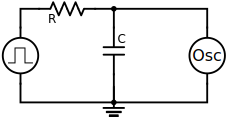
\includegraphics[width=80mm]{schema.pdf}
%    \caption{Schema del circuito utilizzato.}
%    \label{fig:circuito}
%\end{wrapfigure}


\section{Strumenti}

$\bullet \quad$Oscilloscopio \\
$\bullet \quad$Cablaggio\\
$\bullet \quad$Breadboard (basetta sperimentale)\\
$\bullet \quad$Generatore di forme d'onda\\
$\bullet \quad$Multimetro digitale\\
<<<<<<< HEAD
$\bullet \quad$Decadi di resistenze, capacità e induttanze\\
=======
$\bullet \quad$Decadi di resistenze, capacitori e induttanze\\
>>>>>>> 05ca6aaa601c06c868236acb7617353e26b38697
